\chapter{Introduction}
\label{sec:intro}

This thesis is financed by BORDER 6, a interdomain \acf{TE} solution provider for multi-homed stub \acf{AS} and \acf{CDN}. 
It features a platform enabling performance oriented interdomain TE through continuous measurements.
Upon its request, we study in this thesis the various problems encountered in making better use of these available measurements to improve the TE platform from multiple aspects: scalability, measurement interpretation and performance event visibility.

\section{Intradomain Routing and TE}
Internet is interconnection of tens of thousands of independently manged networks known as \acf{AS}.
Routing that happens between those ASes is referred to \textit{interdomain routing}.
The operation of selecting best interdomain routes subject to a specific objective is thus called \textit{interdomain TE}.

In order to exchange interdomain routes, each AS uses \acf{BGP}, a path vector routing protocol, to interface with other ASes.  
Two big type of ASes hence emerge: transit provider and stub AS.
Transit provider refers to ASes that offer routing traffic not originated from nor sent to themselves as a commercial service.
For that purpose, a transit provider announces to its client all the interdomain routes its learns and to its transit providers the routes to its clients.
On the contrary, a stub AS only cares about sending out its own traffic and becoming reachable to others.
Reasonably, they only announce to its transit providers the route to itself in order that the rest of the Internet learns it through its transit providers.

Besides the above transit relationship, peering is another type of route and traffic exchange can happen between two ASes under BGP. Two ASes in peering relationship only exchange with each other the route toward themselves, so that they can directly send to each other the traffic toward their peer without employing a transit provider.
\acf{IXP} is a physical facility that facilitates the establishment of peering relationship.

With either transit or peering relationship, or the two at the same time, an AS can learn multiple routes toward a destination. How to select the best route is then known as \textit{outbound interdomain TE}, since it deals with how traffic is sent out. 


A brief intro to intra-domain routing, BGP, alternatives to BGP such as LISP, overlay networking.
Scope our research under BGP as the routing protocol.

Biblio on the past researches and common practices on interdomain TE with BGP.
Traffic steering method: local pref and prefix split for outbound traffic steering; inbound tricks such as AS-path, community are not certain, and less fine grained. Focus on outbound TE.
System design and route selection methods: common practice (related to policies) and research proposals mainly Akella~\cite{Akella2008}.

Introduce the notion of measurement-based intradomain TE and declare it as the topic and context of this thesis.

\section{Motivations for measurement-based intradomain TE}
To help improve a working system/product for interdomain TE.
What remains to be done or what's the gap between these research proposals and a working system.

\section{Building blocks of measurement-based TE}
The building blocks of the systems and remaining challenges.

\begin{figure}[!htb]
\centering
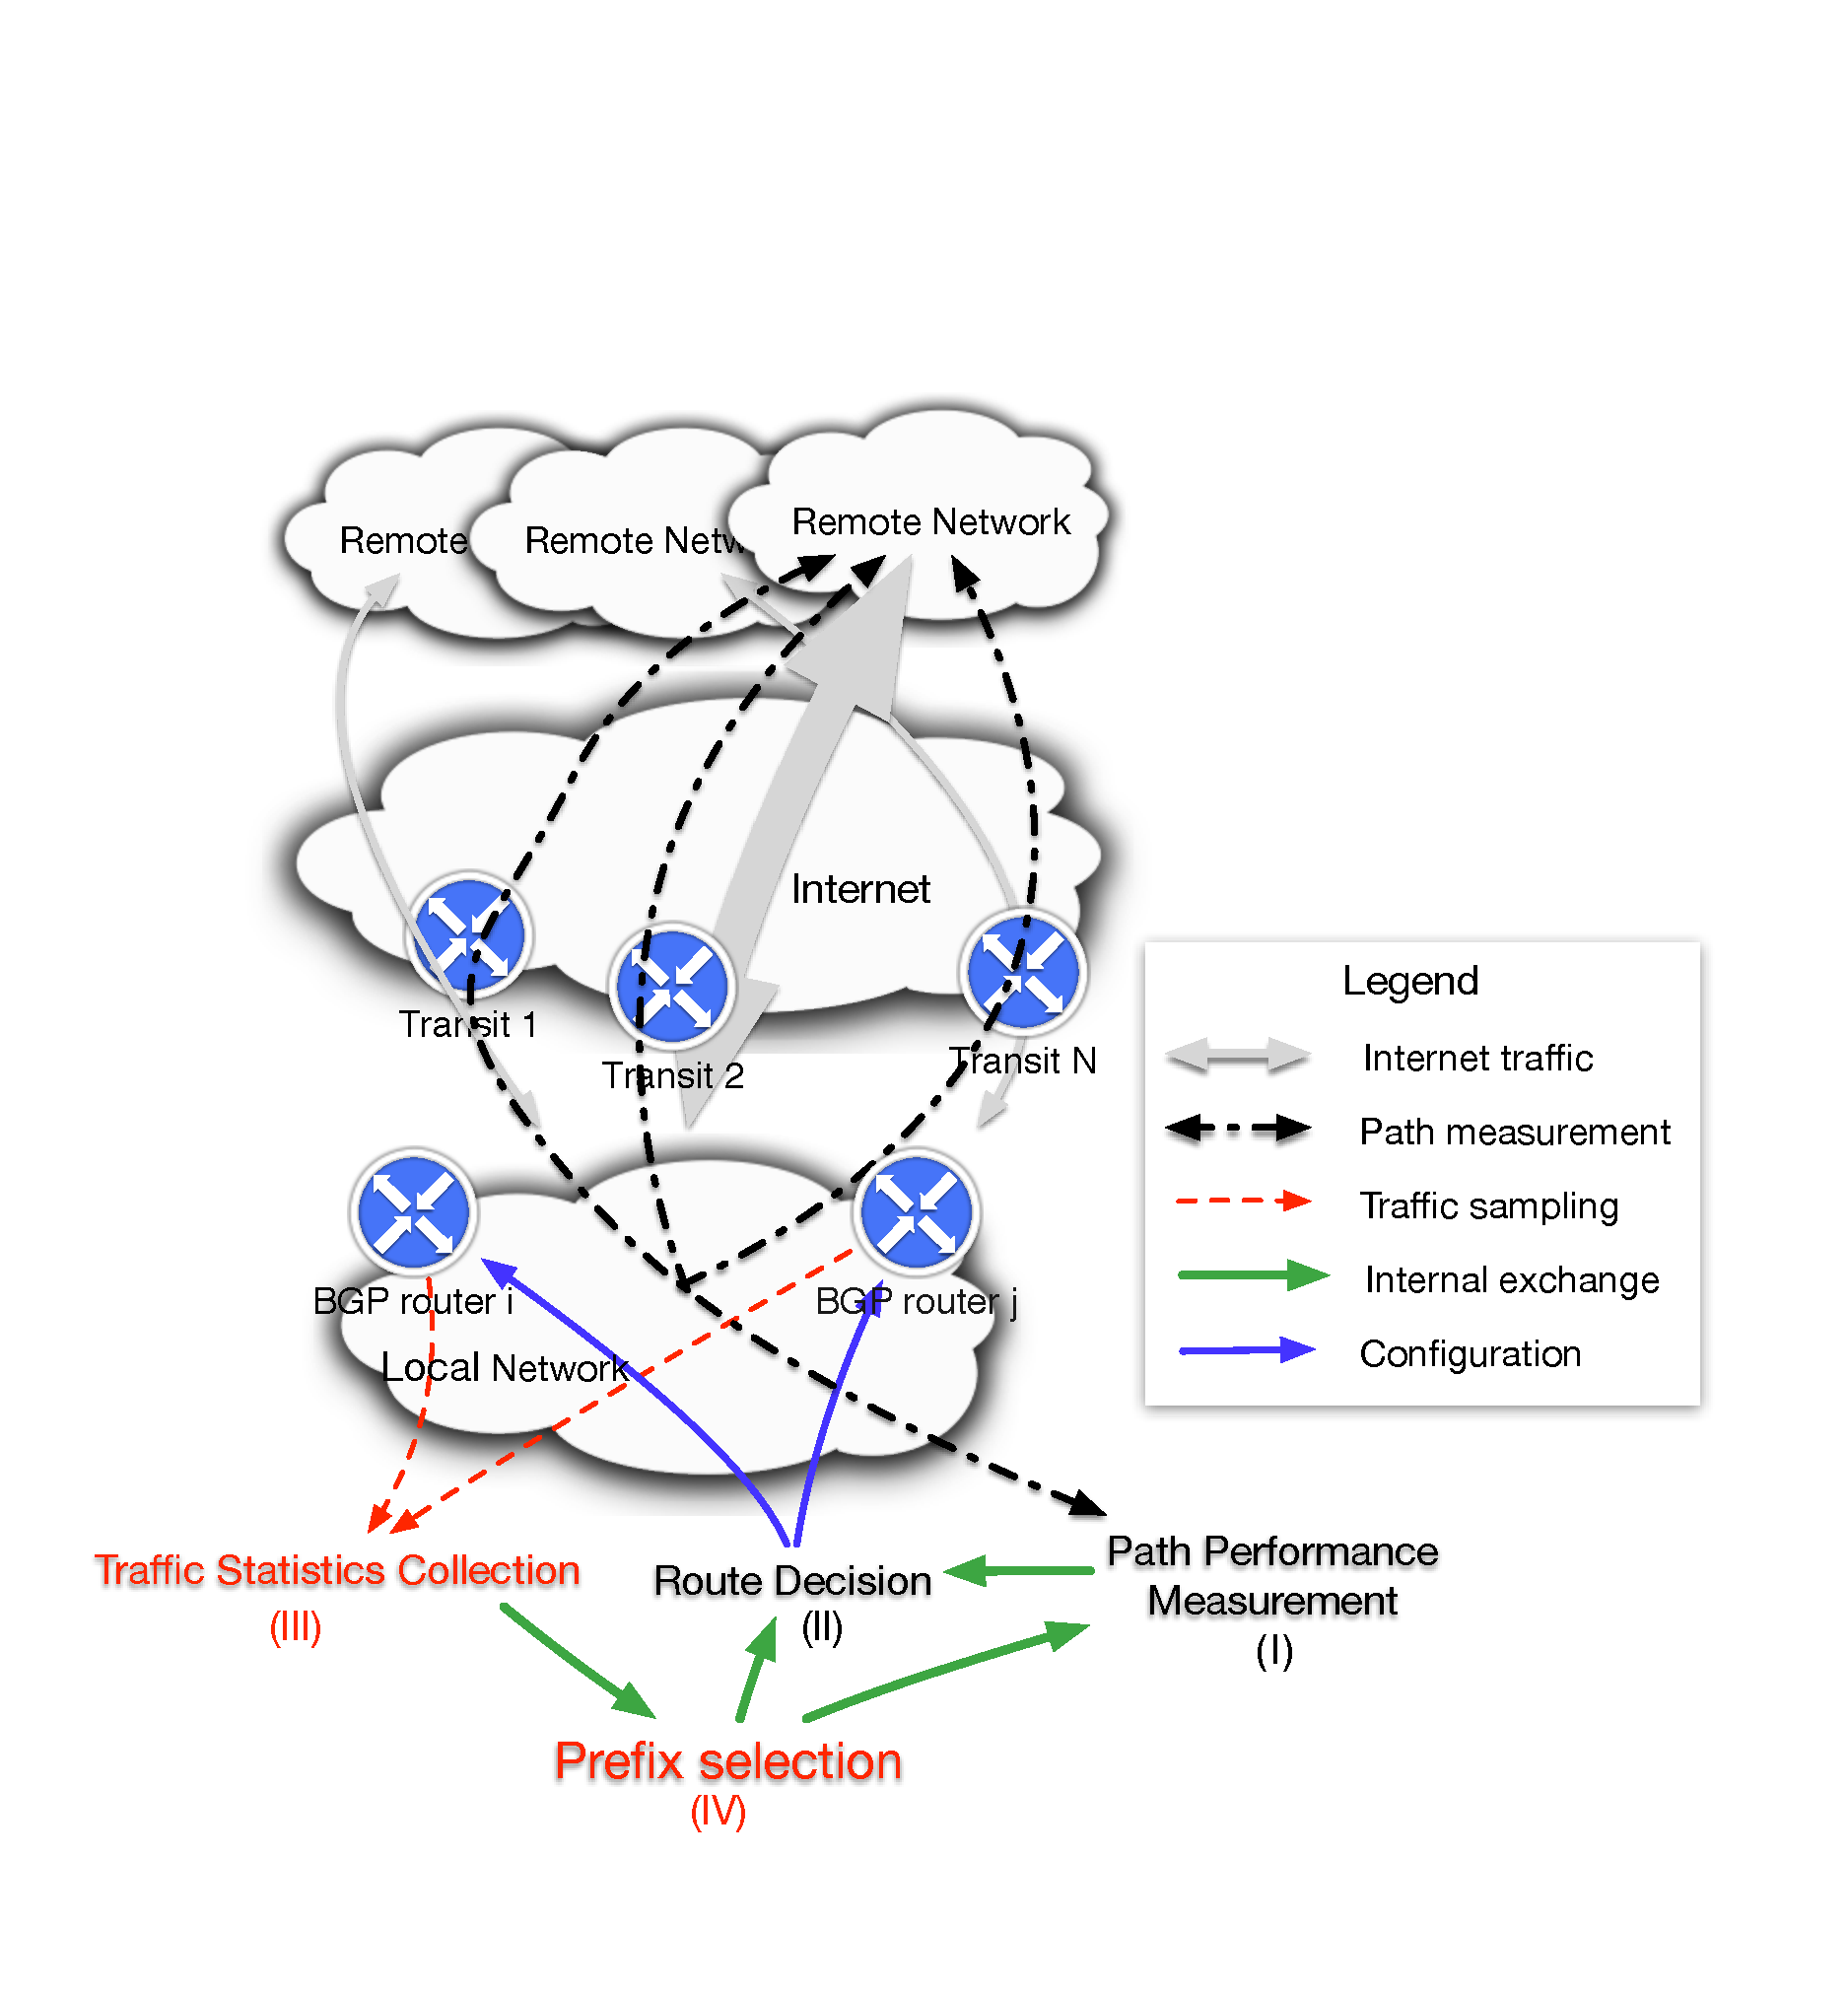
\includegraphics[width=0.9\textwidth]{gfx/chap1/archi.pdf}
\caption{Building blocks of measurement-based inter-domain TE system.}
\label{fig:archi}
\end{figure}

\section{Prefix selection: focus on most important destinations}
Measurements on traffic volumes.
Why we need to focus on most import destinations (a scalability issue), how we did it (NOMS).

\section{RTT measurements with RIPE Atlas}
Measurements on Round-Trip time.
\subsection{RIPE Atlas}
For the sake of reproducibility, use RIPE Atlas as measurement sources.
Intro to RIPE Atlas.
Measurement quality concerning RIPE Atlas.
\subsection{Measurement quality}
Quality issue from the platform (CoNext).
Measurement differences among multiple probes toward a same destination prefix.(AnNet)
Implication to interdomain TE and what we propose.
\subsection{Synchronized RTT change}
Synchronized RTT changes. Time-series clustering.
Motivation for change detection.

\section{Change detection for RTT measurements}
Detect RTT changes (ITC).
Motivation for RTT change detection.

\section{Inferring the location of RTT changes}
The case where probes can not be identified in destination prefixes.
Infer the occurrence of intermediate RTT changes and their locations.
Implication and usage beyond TE.  
